% !TEX root = Projektspezifikation.tex
\section{Middleware}
\subsection{Beschreibung der Middleware}
Aufgabe der Middleware soll es sein die Daten, die in der integrierten Datenbank liegen effizient nach Quellen, Intervallen und weiteren Eigenschaften suchbar zu machen, also einen gezielten und schnellen Zugriff auf Mutationsdaten zu gewährleisten.\\ Hierfür muss sie sowohl in der Lage sein die Einträge aus den Datenbanken zu lesen und aus ihnen eine effizient suchbare Indexstruktur aufzubauen als auch eine Suchfunktionalität bereitstellen, auf die durch die Weboberfläche zugegriffen werden kann. Vom System unterstützte Suchformate sind:
\begin{itemize}
\item Intervallsuche
\begin{itemize}
\item Input: Chromosom, Intervallgrenzen, Quellen und Suchfilter
\item Output: Alle Mutationen, die die vom Nutzer spezifizierten Einschränkungen erfüllen
\end{itemize}
\item Gennamensuche
\begin{itemize}
\item Input: Chromosom, Quellen, Genname
\item Output: alle Mutationen, die die vom Nutzer spezifizierten Einschränkungen erfüllen und die auf dem gesuchten Gen liegen
\end{itemize}
\item Präfixsuche
\begin{itemize}
\item Input: Präfix eines Gennamens
\item Output: alle Gene, die mit dem gesuchten Präfix beginnen
\end{itemize}
\end{itemize} 
Es wird eine Suchstruktur erstellt, in der nach Intervallen gesucht wird und die Mutationsdaten enthält und eine weitere, in der nach Gennamen gesucht werden kann und die Intervallgrenzen für die jeweiligen Gene beinhaltet.
Die Suchstruktur für Intervalle, in der die Mutationsdaten gespeichert werden wird verteilt aufgebaut, um eine effiziente Suche zu ermöglichen.\\
Als Austauschformat mit dem Frontend werden JSON-Nachrichten genutzt. Die Kommunikation mit den Datenbanken erfolgt durch Datenbankzugriffe aus dem Programmcode heraus.\\
Dem Nutzer soll es weiterhin möglich sein die Ergebnisliste zu filtern. Unterstützte Filter sind die Quelldatenbanken in denen gesucht wird, das Chromosom auf dem gesucht wird, Geschlecht, bei der die Mutation auftritt, länderspezifische Herkunft der Mutationsträger und die relative Häufigkeit mit der die Mutation vorkommt.
\begin{figure}[H]
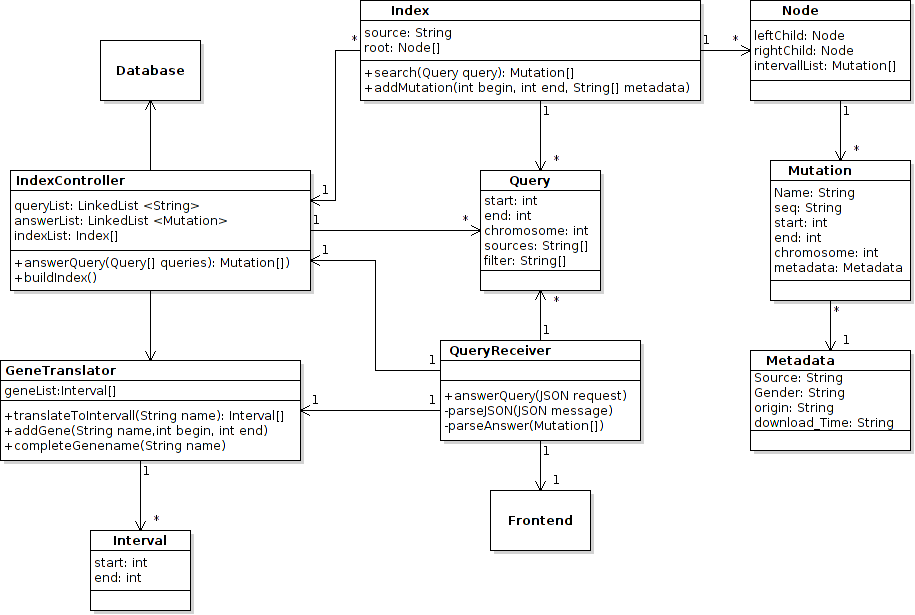
\includegraphics[width=1\textwidth]{middleware/Middleware_Class_final.png}
\caption{Schematischer Aufbau des Systems. Die Kommunikation mit dem Frontend findet über den QueryReceiver statt. Die Kommunikation mit der Datenbank übernimmt der IndexController. Die interne Kommunikation zwischen dem QueryReceiver, dem IndexController und den Indizes finden über Query-Objekte statt, die alle Informationen beinhalten, die für eine Suche benötigt wird. Der IndexController baut sowohl den Mutationsindex, als auch den GeneTranslator auf.}
\end{figure}
\begin{figure}[H]
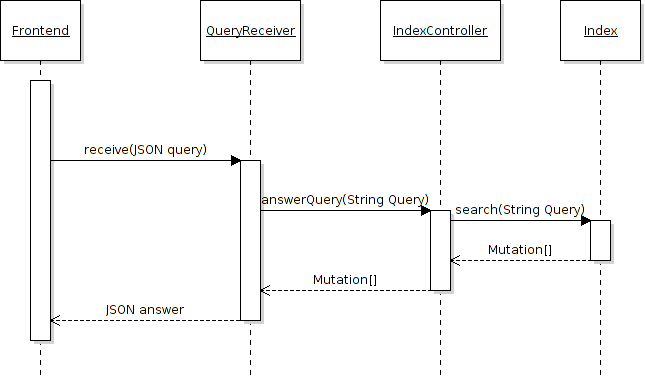
\includegraphics[width=1\textwidth]{middleware/intervall_seq.png}
\caption{Schematischer Ablauf einer Intervallanfrage. Der QueryReceiver erhält eine Anfrage, interpretiert diese und sendet eine Anfrage mit allen nötigen Informationen an den QueryHandler. Dieser ruft mit der Anfrage die Suchfunktionen der Teilindizes auf. Das Ergebnis wird zurückgereicht, ins Antwortformat gepackt und an das Frontend gesendet}
\end{figure}
\begin{figure}[H]
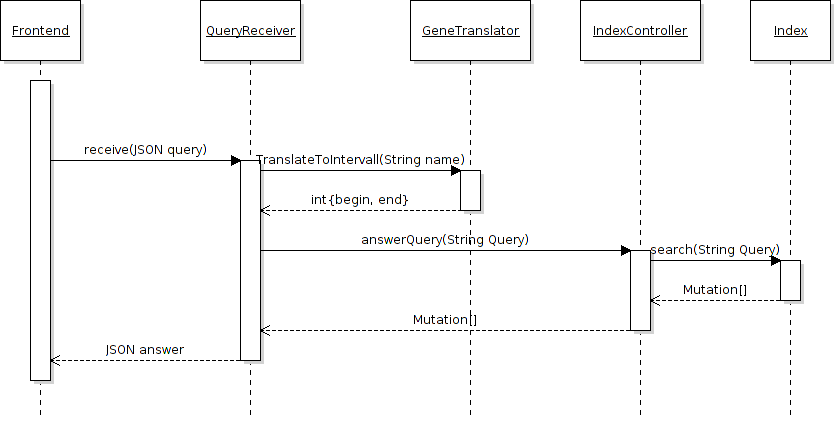
\includegraphics[width=1\textwidth]{middleware/namesearch_seq.png}
\caption{Schematischer Ablauf einer Gennamenanfrage. Nachdem der QueryReceiver die Nachricht erhalten hat schickt er den Gennamen an den GeneTranslator und erhält alle Intervalle, die dem Gen entsprechen. Mit dieser Information wird nun eine Query an den IndexController gestellt. Der weitere Ablauf ist identisch zu dem einer Intervallanfrage.}
\end{figure}
\begin{figure}[H]
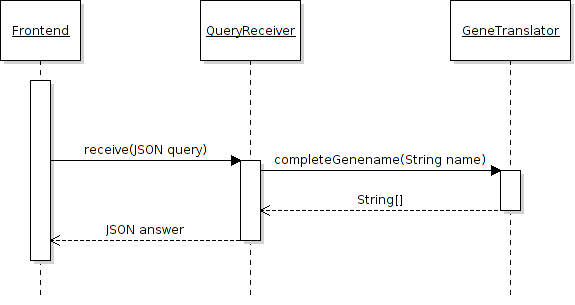
\includegraphics[width=1\textwidth]{middleware/prefix_seq.png}
\caption{Schematischer Ablauf einer Präfixsuche. Der QueryReceiver erhält eine Anfrage und leitet den Genpräfix in der Anfrage an den GeneTranslator weiter. Dieser gibt alle Gene zurück, die mit diesem Präfix beginnen. Die Antwort wird vom QueryReceiver in das Anfrageformat gepackt und an das Frontend gesendet.}
\end{figure}

\subsection{IndexController}
Der Index soll eine effiziente Suche nach Mutationen für das Frontend ermöglichen. Während des Programmstarts wird der Index aus der vorhandenen Datenbank aufgebaut und steht dann so lange zur Verfügung, bis das Programm beendet wird.
Im Index wird mit Intervallgrenzen gesucht und der Index gibt alle Intervalle zurück, die komplett innerhalb des angegebenen Intervalls liegen.\\
Der Index wird verteilt aufgebaut und liegt auf 4 virtuellen Maschinen verteilt. Die für den Index spezifizierten Funktionen sprechen immer einen Teilindex an. Der Aufruf der Funktionen wird über den IndexController erfolgen, der immer alle 4 Teilindizes ansprechen wird.
\subsubsection{Anforderungen}
Der IndexController ist für den Zugriff auf den Gesamtindex verantwortlich. Er nimmt Intervallanfragen entgegen und leitet diese an die Teilindizes weiter.
Die Teilergebnisse, die von den Indizes zurückgegeben werden, werden zusammengeführt und zurückgegeben.
Außerdem baut er zu Programmstart aus der bestehenden Datenbank heraus den Index auf.
\subsubsection{Funktionen}
\begin{itemize}
\item answerQuery(Query[] queries) returns Mutation[] answers\\
Die Funktion erhält eine Liste an Anfragen und gibt eine Liste aller Mutationen zurück, die den Anfrageforderungen entsprechen
\item buildIndex() returns void\\
Die Funktion baut den Index aus der Datenbank auf
\end{itemize}
\paragraph{answerQuery()}
Die Funktion erhält eine Liste an Query-Objekten. Ein Query-Objekt beinhaltet alle nötigen Information zu einer gegebenen Anfrage (gesuchtes Intervall, Quelle, Chromosom, Filterangaben)\\
Die Anfragen werden nebenläufig an die 4 Teilindizes weitergeleitet. Die einzelnen Teilergebnisse werden zusammengefasst und zurückgegeben.\\
\\
\begin{algorithm}
answerQuery()\\
\KwData{Query[] queries}
\KwResult{List of all matching Mutations for all queries}
Query[] queries\;
Index[] indices\;
Mutation[] answers=null\;
\ForAll{$q \in queries$}
{\ForAll{$i \in indices$}
{answers.add(i.search(q))\;}
}
return answers\;
\end{algorithm}


\paragraph{buildIndex()}
Die Funktion wird bei Programmstart ausgeführt und baut auf Basis der Datenbank die 4 Teilindizes auf. Der Zugriff auf die Datenbank erfolgt mithilfe des "JDBC41"-Treibers für "PostgreSQL". Es werden Anfragen der Form "SELECT * FROM Metadaten" und "SELECT * FROM Mutation" an die Datenbank gestellt, um mit den Ergebnissen die Indexstruktur zu befüllen. Wahrscheinlich werden die Anfragen noch geeignet aufgeteilt, da die Zwischenergebnisse sonst unter Umständen zu groß für den Hauptspeicher wären.\\
Für jede Mutation wird zufällig entschieden in welchen Index sie eingefügt wird.\\
Nachdem der Gesamtindex aufgebaut wird, wird der GeneTranslator aus der Datenbank "RefSeq" aufgebaut.
\begin{algorithm}
buildIndex()\\
\KwData{--}
\KwResult{A built index}
connect to mutation\_database\;
ResultSet rs = executeQuery(query1)\;
GeneTranslator j\;
\ForAll{elements e $\in$ rs}
{choose sub index i to insert into\;
i.addMutation()\;}
connect to genename\_database\;
rs = executeQuery(query2)\;
\ForAll{elements e $\in$ rs}
{j.insert(e)\;}
return\;
\end{algorithm}
\newpage

\subsection{Index}
\subsubsection{Anforderungen}
Der Index soll eine effiziente Suche nach Mutationen ermöglichen. Dabei gibt es die Möglichkeiten direkt nach einem Intervall zu suchen oder aber nach allen Mutationen zu suchen, die auf einem bestimmten Gen liegen. Während des Programmstarts wird der Index aus der vorhandenen Datenbank aufgebaut und steht dann so lange zur Verfügung, bis das Programm beendet wird.\\
Im Index wird mit Intervallgrenzen gesucht und der Index gibt alle Intervalle zurück, die sich in irgendeinem Punkt mit dem gesuchten Intervall überschneiden.\\
Der Index wird verteilt aufgebaut und teilt sich auf 4 virtuellen Maschinen auf. Die für den Index spezifizierten Funktionen sprechen immer einen der 4 Teilindizes an. Der Aufruf der Funktionen wird über den IndexController erfolgen, der immer alle 4 Teilindizes ansprechen wird.

\subsubsection{Datenstruktur für den Index}
Die dem Index zugrundeliegende Datenstruktur ist ein Intervallbaum. Dieser ermöglicht effizientes Suchen nach und Einfügen von Intervallen.\\
Hierfür wird die frei zugängliche Bibliothek "IntervalST.java" der Universität Princeton als Grundgerüst verwendet. Die vorgenommenen Änderungen belaufen sich hauptsächlich auf eine Anpassung der verwendeten Datenstrukturen, eine Erweiterung der Suchfunktion um Filter und einen geeigneten Umgang mit Duplikaten (mehrere Mutationen auf demselben Intervall). Außerdem können einige für uns unnötige Funktionen entfernt werden. Die Funktionen addMutation() und search() dienen als Interface zu den in der Bibliothek definierten Funktionen, die Elemente einfügen und suchen\\
Das Suchergebnis wird nach den bei der Anfrage spezifizierten Filtern gefiltert. Bei n Intervallen und einer Such-Ergebnisliste der Größe m ergibt sich ein Komplexität von $\mathcal{O}$(log n + m)\\
\subsubsection{Funktionen}
\begin{itemize}
\item addMutation(Mutation mutation)returns void\\
Die Funktion erhält eine Mutation, die eingefügt werden soll
\item search(Query query)returns Mutation[]\\
Die Funktion erhält eine Anfrage und gibt alle Mutation zurück, die den Anfrageanforderungen entsprechen
\end{itemize}
\newpage
\paragraph{addMutation()}
Die Funktion erhält eine Mutation als Parameter und fügt diese in Indexstruktur ein.
\begin{algorithm}
addMutation()\\
\KwData{Mutation input}
\KwResult{input added to index}
IntervalTree i\;
insert input into i\;
return\;
\end{algorithm}
\paragraph{search()}
Die Funktion erhält eine Anfrage nach dessen Kriterien nach Mutationen gesucht werden soll und einen Knoten des Baumes (zu Beginn der Wurzelknoten). Es werden alle Mutationen gesucht, die komplett oder teilweise innerhalb der Intervallgrenzen liegen. Für alle Mutationen auf die dies zutrifft wird geprüft, ob sie den Filtern entsprechen nach denen gesucht wird. Alle Elemente, die die Filtereinschränkung erfüllen werden zurückgegeben.
\begin{algorithm}
search()\\
\KwData{Query input, Node current}
\KwResult{List of all matching mutations}
IntervalTree i\;
Mutation[] answer\_list\;
{\eIf{current node matches searched interval}
{add mutation to answer\_list if it corresponds to specified filters\;}
{continue search in subtrees\;}}
return answer\_list\;
\end{algorithm}
\newpage

\subsection{GeneTranslator}
\subsubsection{Anforderungen}
Der GeneTranslator wird aufgerufen, falls es sich bei der Anfrage um eine Präfixsuche oder eine Gennamensuche handelt. Die Komponente beinhaltet eine Datenstruktur, die alle im System vorhandenen Gennamen und ihre Intervallbereiche beinhaltet.\\
Die Komponente ermöglicht eine effiziente Suche nach Gen-Präfixen und nach Gennamen um die zugehörigen Intervalle zu erfragen.\\
Als interne Datenstruktur wird ein PatriciaTrie genutzt. Dieser ist in der frei zugänglichen Bibliothek "Apache Commons" vorhanden und wird für diese Implementation genutzt.

\subsubsection{Funktionen}
\begin{itemize}
\item translateToInterval(String name) returns Intervall[]\\
Die Funktion erhält einen Gennamen, nach dem gesucht wird und gibt eine Liste von Intervallobjekten zurück, die den Start-und den Endpunkt aller Vorkommen des Gens beinhalten
\item addGene(String name, int begin, int end) returns void\\
Die Funktion erhält einen Gennamen und die Intervallgrenzen des Gens und fügt diese in die zur Suche benötigten Datenstruktur ein
\item completeGenename(String name) returns String[]\\
Die Funktion erhält einen Präfix eines Gennamens und gibt alle Gennamen zurück, die mit diesem Präfix beginnen
\end{itemize}
\paragraph{translateToInterval()}
Diese Funktion wird aufgerufen, falls eine Gensuche angefragt wird. Sie überstetzt das gesuchte Gen in die zugehörigen Intervalle um eine Intervallsuche aus der Anfrage zu machen, die vom Index bearbeitet werden kann.

\paragraph{addGene()}
Die Funktion fügt der internen Datenstruktur ein Gen und die zugehörigen Intervalle hinzu. Sollte sich das Gen bereits in der Struktur befinden, so wird überprüft, ob eines der vorhandenen Intervalle für diesen Gen komplett im neu hinzugefügten befindet. Ist dies der Fall, so wird das alte Intervall durch das neue ersetzt. Andernfalls wird das neue Intervall an die Liste der Intervalle für dieses Gen zugefügt. Sollten die Intervalle eines Gens komplett denen eines anderen Gens entsprechen, so kann davon ausgegangen werden, dass diese synonyme Bezeichnungen für das gleiche Gen sind. Da die Intervalle bereits gleich sind werden Synonyme implizit abgefangen.

\paragraph{completeGenename()}
Die Funktion gibt alle Gennamen zurück, die mit dem gesuchten Präfix beginnen\\
\newpage

\subsection{QueryReceiver}
\subsubsection{Anforderungen}
Der QueryReceiver bildet die direkte Schnittstelle zum Frontend. Alle Anfragen, die der Nutzer eingibt werden als JSON-File an ihn gesendet und Antworten werden von ihm an das Frontend zurückgegeben. Die Komponente überprüft für alle eingehenden Anfragen um was für eine Anfrage-Art es sich handelt und leitet sie an die zuständigen Teilkomponenten weiter.\\
Für die einzelnen JSON-Formate siehe Abschnitt Schnittstelle GUI-Middleware\\

\subsubsection{Funktionen}
\begin{itemize}
\item answerQuery(JSON request) returns JSON answer\\
Die Funktion erhält eine Anfrage im JSON-Format und gibt eine Antwort im JSON-Format zurück
\end{itemize}
\paragraph{answerQuery()}
Alle Nutzer-Anfragen werden an diese Funktion gesendet. Sie überprüft anhand des Aufbaus der JSON-Anfrage, um was für eine Anfrageart es sich handelt.\\ Bei der Intervallsuche wird die JSON-Anfrage in ein Query-Objekt umgewandelt und an den IndexController weitergeleitet. Bei der Gennamensuche wird zuerst im GeneTranslator nach dem zum Gen gehörigen Intervall gesucht und mit dieser Information und den Filterangaben des Nutzers ein Query-Objekt erstellt, dass dem IndexController übergeben wird. Handelt es sich um eine Präfixsuche wird im Genetranslator nach Gennamen gesucht, die mit dem Präfix beginnen. Die Antworten der jeweiligen Anfragen werden in das zum Anfragetyp gehörende JSON-Antwortformat verpackt und an das Frontend zurückgesendet.\\

\newpage
\section{Stresstest}
Der Stresstest hat zum Ziel herauszufinden, wie lange die durchschnittliche Query-Laufzeit ist.\\
Ziel des Systems ist es eine Laufzeit von unter einer Sekunde zu erreichen.\\
Um dies zu überprüfen werden zufällig je 50 korrekte Anfragen der gleichen Art (Intervallsuche, Gennamenssuche, Präfixsuche) an das System gestellt und die Antwortzeiten gemessen. Diese dürfen alle nicht länger als eine Sekunde zur Antwort brauchen.\\
Hierfür wird ein Testprogramm geschrieben, dass Anfragen im korrekten Format stellt und die Antwortzeiten automatisch auswertet. Die Anfragen werden zufällig generiert.

\newpage
\subsection{Unit-Tests}
\subsubsection{QueryReceiver}
\textbf{Testfall 1 - erfolgreiche Intervallanfrage ohne Metadaten}
\begin{verbatim}
  Eingabe
{
  "source": The Cancer Atlas,\usepackage[utf8]{inputenc}
  "chromosome": 3,
  "position": {"from": 100, "to": 200},
  "zoom": 1,
  "subindex": ,
  "hasDetail": (false)
}

  Ausgabe
{
  {
    "source:" The Cancer Atlas,
    "chromosome": 3,
    "position": {"from": 100, "to": 200},
    "details": { "refseq": ,
                "mutations": [{ "name": ,
                                "position": {"from": , "to": },
                                "metadata":
                              },]},
    "graph": {
              { "subintervall": Anzahl der Subintervalle,
                "counts": Anzahl der Ergebnisse
              }
            }
  }
}
\end{verbatim}
\textbf{Testfall 2 - erfolgreiche Intervallanfrage mit Metadaten}
\begin{verbatim}
  Eingabe
{
  "source": The Cancer Atlas,
  "chromosome": 3,
  "position": {"from": 100, "to": 200},
  "zoom": 1,
  "subindex": ,
  "hasDetail": (true)
}

  Ausgabe
{
  {
    "source:" The Cancer Atlas,
    "chromosome": 3,
    "position": {"from": 100, "to": 200},
    "details": { "refseq": Referenzsequenz,
                "mutations": [{Mutation1},{Mutation2},...]},
    "graph": {
              { "subintervall": ,
                "counts":
              }
            }
  }
}
\end{verbatim}
\textbf{Testfall 3 - Intervallanfrage mit leerer Antwortmenge}
\begin{verbatim}
  Eingabe
{
  "source": The Cancer Atlas,
  "chromosome": 3,
  "position": {"from": 100, "to": 200},
  "zoom": 1,
  "subindex": ,
  "hasDetail": (true)
}

  Ausgabe
{
  {
    "source:" The Cancer Atlas,
    "chromosome": 3,
    "position": {"from": 100, "to": 200},
    "details": { "refseq": ,
                "mutations": ...},
    "graph": {
              { "subintervall": ,
                "counts":
              }
            }
  }
}
\end{verbatim}
\newpage\hfill\\
\textbf{Testfall 4 - erfolgreiche Namensanfrage}
\begin{verbatim}
  Eingabe
{
  "source": The Cancer Atlas,
  "chromosome": 3,
  "search": "Gen im Cancer Atlas"
}

  Ausgabe
{
  "source": The Cancer Atlas,
  "chromosome": 3,
  "search": "Gen im Cancer Atlas",
  "position": {"from": Startposition, "to": Endposition}
}
\end{verbatim}
\textbf{Testfall 5 - Namensanfrage mit leerer Antwortmenge}
\begin{verbatim}
  Eingabe
{
  "source": The Cancer Atlas,
  "chromosome": 3,
  "search": "Gen, dass nicht im Cancer Atlas ist"
}

  Ausgabe
{
  "source": The Cancer Atlas,
  "chromosome": 3,
  "search": "Gen im Cancer Atlas",
  "position": " "
}
\end{verbatim}
\textbf{Testfall 6 - fehlerhafte Anfrage}
\begin{verbatim}
  Eingabe
{
  "source": ""
}

  Ausgabe
{
  "answer": "unknown format"
}
\end{verbatim}
\newpage
\subsubsection{GeneTranslator}
Der GeneTranslator hat 2 Aufgaben. Zum einen soll er während der Indexerstellung mit Inhalt (also Gennamen und zugeörigen Intervallen) befüllt werden, zum anderen soll eine Suche nach Gennamen in ihm möglich sein.\\
\\
\textbf{Testfall 1 - addGene - Einfügen in Datenstruktur}\\
Eingabe: Testgen, 350, 500\\
Ausgabe: Dass Gen sollte in den Baum eingefügt sein und per searchForGene() findbar sein\\
\\
\textbf{Testfall 2 - addGene - Doppeltes Einfügen in Datenstruktur}\\
Eingabe: Testgen, 350, 500\\
		 Testgen, 350, 500\\
Ausgabe: Dass Gen sollte nur einmal in die Datenstruktur eingefügt werden. Ausgabe, dass das Gen bereits in der Struktur vorhanden ist.\\
\\
\textbf{Testfall 3 - addGene - Aufruf ohne Parameter}\\
Eingabe: [...]\\
Ausgabe: Fehlermeldung über  parameterlosen Aufruf\\
\\
\textbf{Testfall 4 - tranlateToIntervall - erfolgreiche Suche}\\
Eingabe: Testgen (befindet sich bereits in Datenstruktur)\\
Ausgabe: 350, 500\\
\\
\textbf{Testfall 5 - tranlateToIntervall - erfolglose Suche}\\
Eingabe: Testgen2 (befindet sich nich in Datenstruktur)\\
Ausgabe: Fehlermeldung über erfolglose Suche\\
\\
\textbf{Testfall 6 - tranlateToIntervall - Aufruf ohne Parameter}\\
Eingabe: [...]\\
Ausgabe: Fehlermeldung über Parameterlosen Aufruf\\
\\
\textbf{Testfall 7 - completeGeneName - erfolgreiche Suche mit einem Ergebnis}\\
Eingabe: Test (Testgen1 befindet sich bereits in Datenstruktur)\\
Ausgabe: Testgen1\\
\\
\textbf{Testfall 8 - completeGeneName - erfolgreiche Suche mit mehreren Ergebnissen}\\
Eingabe: Test (Testgen1 und Testgen2 befinden sich bereits in Datenstruktur)\\
Ausgabe: Testgen1, Testgen2\\
\\
\newpage\hfill\\
\textbf{Testfall 9 - completeGeneName - erfolglose Suche}\\
Eingabe: Test (Es befindet sich kein Gen mit Präfix Test in der Datenstruktur)\\
Ausgabe: Fehlermeldung über erfolglose Suche
\subsubsection{IndexController}
\textbf{Testfall 1 - answerQuery - einfache Intervallanfrage}\\
Eingabe: 1,3,100,200\\
Ausgabe: zum Intervall gehörende Mutationsobjekte\\
\\
\textbf{Testfall 2 - answerQuery - komplexere Intervallanfrage}\\
Eingabe: 1,3,100,200 ; 1,3,150,350\\
Ausgabe: eine Mutationsliste mit den Ergebnissen beider Anfragen\\
\\
\textbf{Testfall 3 - answerQuery - unvollständige Intervallanfrage}\\
Eingabe: 1,100,200\\
Ausgabe: Fehlermeldung über unvollständige Anfrage\\
\\
\textbf{Testfall 4 - answerQuery - leere Anfrage}\\
Eingabe: [...]\\
Ausgabe: Fehlermeldung über leere Anfrage\\
\\
\textbf{Testfall 5 - answerQuery - überspezifizierte Intervallanfrage}\\
Eingabe: 1,3,100,200,300,400\\
Ausgabe: Fehlermeldung über überspezifizierte Anfrage\\
\\
\textbf{Testfall 6 - buildIndex - erfolgreicher Indexaufbau}\\
Eingabe: [...] (Datenbank ist erreichbar)\\
Ausgabe: Erfolgreich gebauter Index\\
\\
\textbf{Testfall 7 - buildIndex - erfolgloser Indexaufbau}\\
Eingabe: [...] (Datenbank ist nicht erreichbar)\\
Ausgabe: Fehlermeldung über erfolglosen Indexaufbau
\newpage
\subsubsection{Intervallbaum}
\textbf{1. Intervalle einfügen:}\\
Das Intervall muss im Baum an der richtigen Stelle eingefügt werden und der Baum muss gegebenenfalls neu balanciert werden (z.B. wie ein AVL-Baum).\\\\
Bsp.: Einfügen des Intervalls [12,15]
\begin{figure}[H]
 \centering
	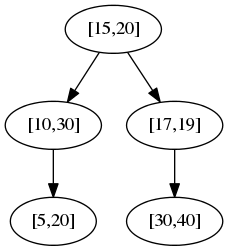
\includegraphics[width=0.2\textwidth]{middleware/Testfaelle/1.png}
	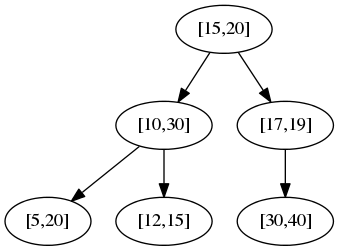
\includegraphics[width=0.3\textwidth]{middleware/Testfaelle/2.png}
\end{figure}
\textbf{2. Intervall mit Startpunkt $>$ Endpunkt einfügen:}\\
Wenn ein Intervall (S,E) mit S$>$E eingefügt wird, dann sollte unser Programm eine Fehlermeldung ausgeben und darauf hinweisen, dass die Grenzen für das Intervall nicht korrekt sind.\\\\
Bsp.: Einfügen des Intervalls [20,10] in einen beliebigen Baum.\\\\
\textbf{3. Intervall mit Start- bzw. Endpunkt außerhalb des betrachteten Zahlenbereichs:}\\
Wenn ein Intervall in dem Baum eingefügt werden soll, das teilweise oder vollständig außerhalb unseres Zahlenbereichs liegt (Länge des Genoms), dann muss es eine Fehlermeldung geben, die dem Nutzer mitteilt, dass der gültige Zahlenbereich überschritten wurde.\\\\
Bsp.: Einfügen des Intervalls [-5,7] in einen beliebigen Baum.\newpage\hfill\\
\textbf{4. Schon vorhandenes Intervall einfügen:}\\
Duplikate sollen von unserem Baum nicht gespeichert werden, d.h. es wird kein neuer Knoten hinzugefügt, sondern die Informationen (bei uns also Pointer auf Dateien) des neuen Knotens müssen im bereits vorhandenen Knoten mitgespeichert werden.\\\\
Bsp.: Einfügen des Intervalls [15,20] in den folgenden Baum\\\\
\includepicture[width=0.2\textwidth]{middleware/Testfaelle/1.png}{ }
\textbf{5. Suche nach vorhandenem Intervall:}\\
Bei der Suche sollen alle Intervalle ausgegeben werden, die das gesuchte Intervall in irgendeinem Punkt überlappen.\\\\
Bsp.: Suche im folgenden Baum\\\\
\includepicture[width=0.3\textwidth]{middleware/Testfaelle/2.png}{ }
Suche [4,5] $\Rightarrow$ gib [5,20] aus\\
Suche [25,35] $\Rightarrow$ gib [10,30] und [30,40] aus\\
Suche [20,20] $\Rightarrow$ gib [15,20] und [5,20] aus
\subsection{Stresstests}
Der Stresstest hat zum Ziel herauszufinden, wie lange die durchschnittliche Query-Laufzeit ist.\\
Ziel des Systems ist es eine Laufzeit von unter einer Sekunde zu erreichen.\\
Um dies zu überprüfen werden mehrere Anfragen der gleichen Art (Intervallsuche, Gennamenssuche, Präfixsuche) sequentiell gestellt und die Antwortzeit gemessen. Alle Anfragen sollen in unter einer Sekunde eine Antwort erzielen.

